% SPDX-FileCopyrightText: 2023 Iegor Riepin, Tom Brown
%
% SPDX-License-Identifier: CC-BY-4.0

\subsection{Methods and tools} 

The simulations were carried out with the open-source software PyPSA for energy system modelling \cite{horschPyPSAEurOpenOptimisation2018} and Linopy for optimization \cite{LinopyLinearOptimization2024}.
The mathematical model is a system-wide cost-minimisation problem. 
The objective of the model is to co-optimise (i) investment and dispatch decisions of generation and storage assets done by datacenters to meet their electricity demand in line with 24/7 CFE objectives, (ii) space-time load-shifting decisions subject to datacenter flexibility constraints, as well as (iii) investment and dispatch decisions of assets in the rest of the European electricity system to meet the demand of other consumers.
The model formulation includes the the linear optimal power flow approximation on the transmission network. 
This work uses a brownfield investment approach, which means that the model includes information about the existing assets of the European electricity system. 

The electricity system dispatch and investment problem of this type is a standard in the energy modelling literature \cite{OpenModelsWikib}, the clean computing model is based on the framework of 24/7 CFE accounting suggested by Google \cite{google-methodologies} that was implemented in realms of energy system models by Xu et al. \cite{xu-247CFE-report} and Riepin \& Brown \cite{riepinMeansCostsSystemlevel2023}, and the space-time load flexibility model is inspired by the work of Zhang et al. \cite{zhangRemuneratingSpaceTime2022} The space-time load flexibility as a degree of freedom within the 24/7 CFE matching problem is a novel contribution of this work.


\subsection{Datacenter model} 

Datacenters are represented as a subset of demand nodes for electricity with a fixed demand profile, controlled degree of flexibility, and a set of specific constraints ensuring the carbon-free energy matching and utilisation of flexibility in a feasible domain.


\begin{figure}
    \centering
    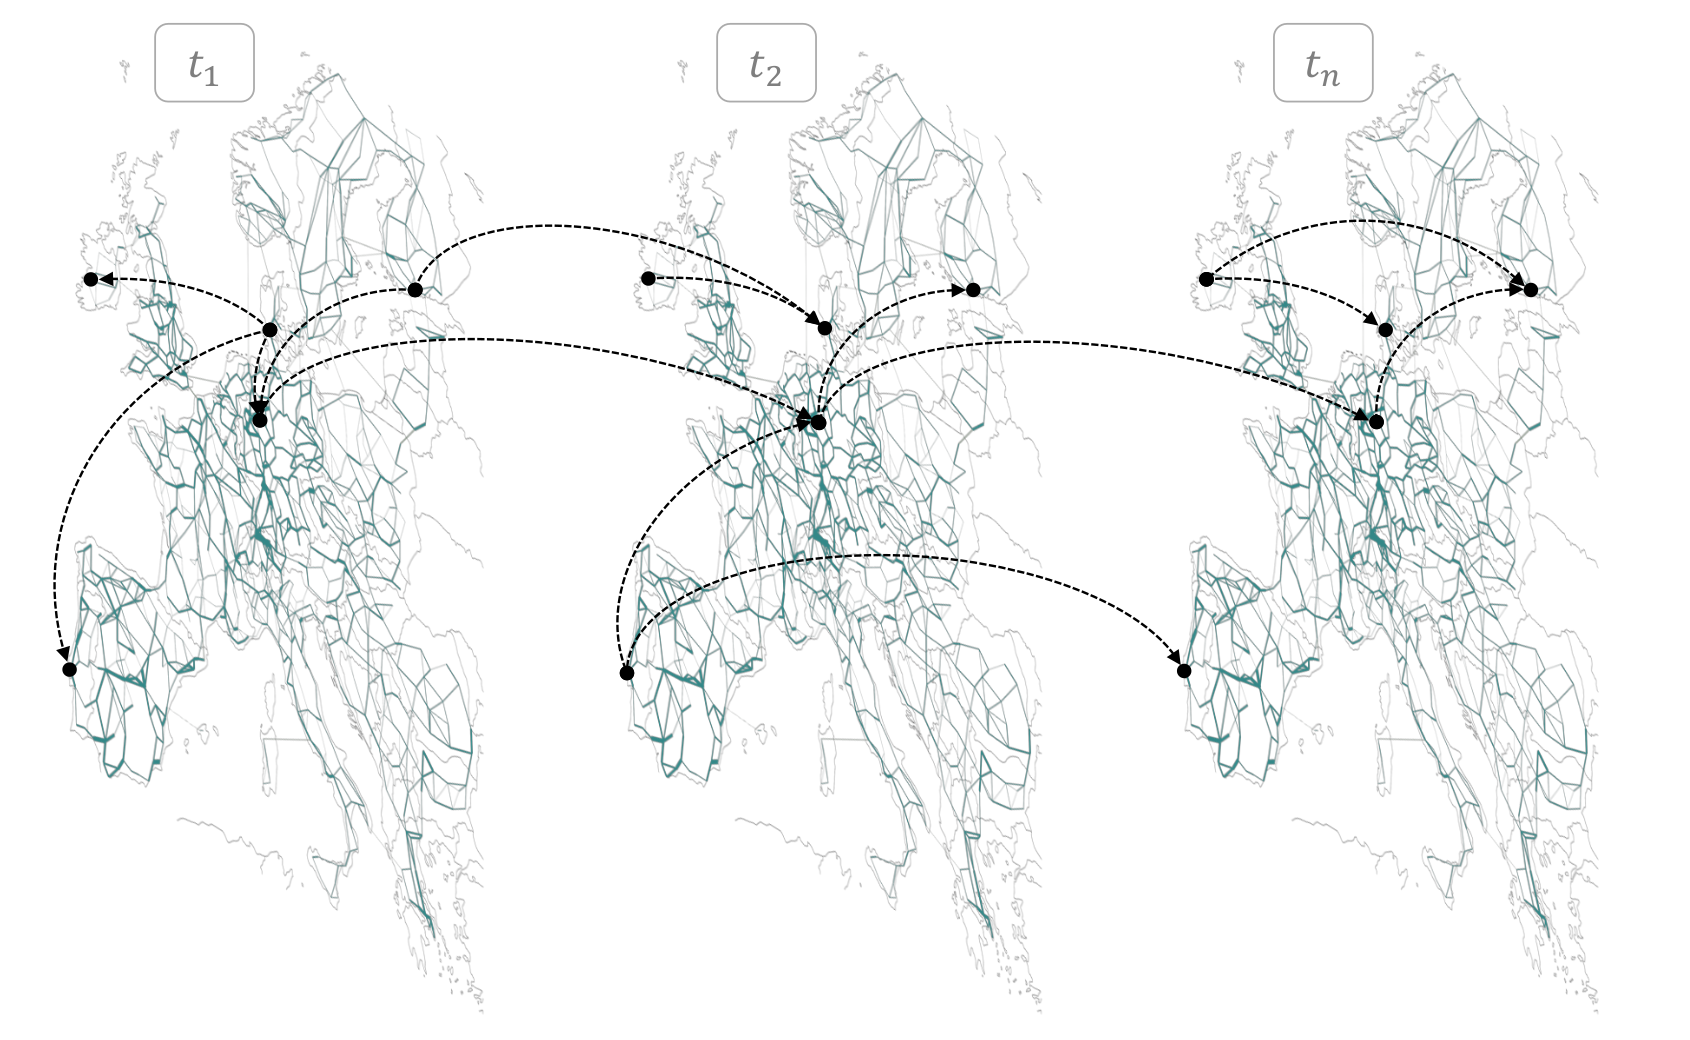
\includegraphics[width=0.95\columnwidth]{img/datacenter-problem.png}
    \caption{Illustration of spatio-temporal load-shifting optimisation problem faced by a datacenter operator.}
    \label{fig:space-time-optimisation}
\end{figure}

% 24/7 CFE 

The 24/7 CFE matching problem introduces a set of new model components (parameters, variables, constraints) into the power system optimisation problem to represent voluntary yet binding carbon-free energy matching commitments. Here, we model a situation where one company operating a network of datacenters that are geographically distributed but managed collectively. The company is committed to match every kilowatt-hour of electricity consumption by carbon-free sources in all datacenter locations. To achieve the target, the company optimises its procurement of carbon-free generation and storage resources and operational decisions, such as dispatch of procured assets, load-shifting flexibility use, imports of electricity from the regional grid, and when necessary, curtailment of excess generation.

\textbf{A case of single datacenter with inflexible load --} First, consider a case of a single datacenter with demand profile $d_{t}$ for each hour $t$ of the year. The demand profile is assumed to be known in advance and is not flexible. In such case, energy balance constraint requires that hourly demand is met by a combination of the following: (i) dispatch $g_{r,t}$ of procured carbon-free generators $r\in CFE$, (ii) dispatch $\bar{g}_{s,t}$ of procured storage technologies $s\in STO$, and (iii) imports of electricity from the regional grid $im_{t}$:

\begin{equation}
    \begin{split}
        \sum_{r\in CFE} g_{r,t} &+ \sum_{s\in STO} \left(\bar{g}_{s,t} - \underline{g}_{s,t}\right) - ex_t + im_t = d_t \quad \forall t \in T
    \end{split}
\label{eqn:CFE}
\end{equation}

Note that if total electricity yield of renewable generators procured by datacenter operator exceeds demand in a given hour, the excess electricity $ex_t$ has to be either stored or curtailed.\footnote{In practice, excess electricity can also be sold to the regional electricity market at wholesale market prices. This option is deliberately avoided in this work.}

The 24/7 CFE matching constraint requires that sum over hourly generation from the contracted generators, plus net dispatch of the storage technologies, plus imports of electricity from the regional grid multiplied by the grid's hourly CFE factor $CFE_t$ minus the excess electricity must be higher or equal than a certain CFE score $x$ multiplied by the total load of a datacenter:

\begin{equation}
    \begin{split}
        \sum_{r\in CFE, t\in T} g_{r,t} &+ \sum_{s\in STO, t\in T} \left(\bar{g}_{s,t} - \underline{g}_{s,t}\right) \\
        &- \sum_{t\in T} ex_t + \sum_{t\in T} CFE_t \cdot im_t \geq x \cdot \sum_{t\in T} d_t
    \end{split}
\label{eqn:CFE}
\end{equation}

% On CFE target
\noindent where \textit{CFE score} $x$[\%] measures the degree to which hourly electricity consumption is matched with carbon-free electricity generation. \cite{google-methodologies} Thus, equation (\ref{eqn:CFE}) allows for controlling \textit{the quality score} of the 24/7~CFE procurement by adjusting the parameter $x$, which was subject of research in recent literature. \cite{riepinMeansCostsSystemlevel2023,xu-247CFE-report} Here, we focus on the best quality score ($x=1$) ensuring that every kilowatt-hour of electricity consumption is met by carbon-free sources at all times.

Note the following properties of the 24/7 CFE matching problem:

\begin{enumerate}
    \item The contracted generators $r\in CFE$ must be additional to the system and can be sited only in the local bidding zone, known as requirements for \textit{additionality} and \textit{locational matching}.
    \item Excess electricity is not counted toward the CFE score and thus subtracted from the left-hand side of eq. (\ref{eqn:CFE}).
    \item The CFE factor of the regional grid ($CFE_t$) can be seen as the percentage of clean electricity in each MWh of imported electricity to supply demand of participating consumers in a given hour.
    To compute $CFE_t$, we consider both the hourly electricity mix in the local bidding zone and emission intensity of imported electricity from the neighbouring zones.
    The numerical simulations show that for the perfect 24/7 CFE matching ($x=1$), datacenter operator does not rely on electricity imports from the regional grid because local electricity mix must have a strictly zero carbon content for imported electricity to be counted as \enquote{carbon-free}. 
    Thus, datacenter operator has one less degree of freedom to meet the 24/7 CFE matching target.
    The methodology to calculate the grid CFE factor and lineraise resulting nonconvexity is described in detail in the prior work of the authors \cite{riepin-zenodo-systemlevel247}.
\end{enumerate}

